
\chapter[Mortgage Model]{Mortgage Model}

Individuals qualify for some size of mortgage at a particular borrowing rate. 
 
\section{Mortgage availability} \label{section-mortgage-availability}
The borrowing of most agents will be constrained. A common rule is that mortgage payments cannot exceed some fraction of disposable income. The wealthy will be able borrow larger amounts and at lower interest rates than the less wealthy.

Many personal finance experts recommend total housing costs account for less than 28\% of \textbf{gross} household income, This gives us an \textbf{income-based  mortgage maximum} of 

\[M^{max}_Yi = \frac{0.28*(\omega+w)}{r_i}\] It is the maximum the bank will let you pay.

We assume $r_i$ is based on the individual's assets, on relative wealth. Where is it calculated for the householder or the bank?

We also have  a \textbf{price-based mortgage maximum} \[M^{max}_P = 0.8P_0\] where $P_0$ is the actual sale price. This is based on the maximum amount of risk that the bank is willing to take on. Combining these conditions, %($P_0$  will not always be the same as the asking price or the warranted price.)

\[M^{max}_Yi = min\left\{\frac{0.28*(\omega+w)}{r_i},  0.8P_0 \right\} \]


% \subsection{The cost of capital}
% The cost of capital is known to differ for rich and poor. This model ties the individual cost of capital,  $r_i$ for agent $i$, to a prime rate, $\bar r$, and to individual wealth. Figure~\ref{fig-borrowing-cost} illustrates the cost of the borrowing model we implement, 
%  \[ r_i = (A + B \frac{\bar{W}}{W_i})\omega\]
% Where $\bar{W}$ is mean wealth and $W_i$ is individual wealth. 

If the expected return on a property is greater than the individual cost of borrowing, it would pay any agent to borrow as much as possible and purchase properties as they can available.\footnote{As pointed out above,  Equation~\ref{eqn-property-investment-return2} implies a `bang-bang' control---with all sales going to the richest participant unless there are limits on the size of capital flows. For our simulation, we implement such limits.} 
 

\section{Maximum mortgage calculation}
The bank puts two  limits on the size of the mortgage, one based on income (a \textbf{carrying constraint}) and one based on wealth (a \textbf{wealth constraint}).

% Mortgage gives 2 numbers. First it pays for a share of the purchase price, second it has an actual maximum. 


\begin{figure}
\centering
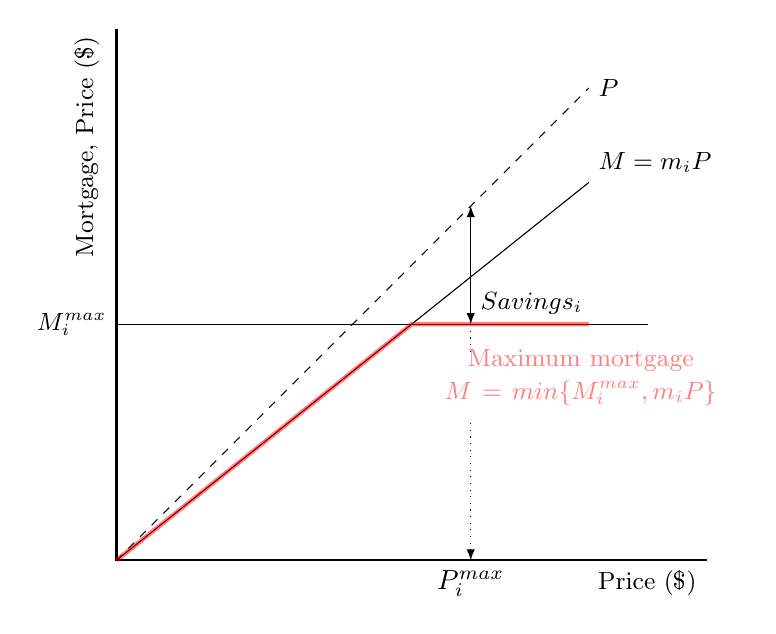
\begin{tikzpicture}	[scale=1.5]
%AXES
\draw[thick] (0,4.5) --(0,0)--(5,0)node[below left]{\small Price (\$)};
\node at (-.25, 3.5)[ rotate=90]{\small Mortgage, Price (\$)};
% M =Mi MAX
\draw[dashed] (0,0)--(4,4)node[right]{\small $P$};
\draw[] (0,2)node[left]{\small $M_i^{max}$}--(4.5,2);%node[right, red]{\small $M = M_i^{max}$};
% M =mi MAX
\draw[] (0,0)--(4,3.2)node[above right]{\small $M = m_iP$};
% COMBINED MAX RED
\draw[ultra thick, red, opacity=.5] (0,0)--(2.5,2)node[below right,  text width=4cm, align = center]{\small \\ Maximum mortgage \\ $M=min\{M_i^{max}, m_iP\}$}--(4.0,2);
% SAVINGS
\draw[latex-latex] (3,2)node[above right] {\small $Savings_i$}--(3,3);
% PMAX
\draw[dotted,latex- ] (3,0)node[below] {$P_i^{max}$}--(3,1.2);
\draw[dotted ] (3,2)--(3,1.72);
\end{tikzpicture}
\caption{The bank's dual mortgage constraint and the savings constraint determine the maximum bid price}
\label{fig:my_label2}
\end{figure}


The two constraints on  mortgage size that the bank imposes are incorporated in the kinked red line in Figure~\ref{fig:Wealth-based}. The maximum  permitted mortgage is combined with the savings constraint to determine the maximum price that a potential home buyer can offer.   

% a kink because there are 2 constraints.  The actual mortgage must be below both lines.
The diagonal line, the top dashed diagonal line, is just the price, P = mortgage + savings.
The difference between the two diagonal lines is what the purchaser pays from savings.  
% This is just the constraint. Up to the kink, little $m_i$ is a fraction of price. beyond at little mi becomes a different number - number based on little $m_i$ for everyone
% banks have an advantage since they can practically bid anything
% m - mortgage share
% P - realized price
% M - maximum - 

\subsection{Wealth-based mortgage maximum} 
\begin{align}
m_i^{max\_permitted} = \mathrm{max\_mortgage\_share} - \left(\frac{W_i}{\bar W}\right)^{\mathrm{wealth\_sensitivity}} \label{eqn-wealth-based-mortgage}    
% m_i^{max\_permitted} = 0.9 - \left(\frac{W_i}{\bar W}\right)^{0.1} 
\end{align} 

% **Source**: Ch:model line 580, page 87.. I have done some fiddling Wealth $W_i = P-M+S.  for i - real estate agents estimated price wealth of a property owner as assessed by the bank.
% Where 0.9 is the maximum fraction that can be mortgaged and 0.1 is the wealth sensitivity parameter.

According to the Canada Housing Statistics Program (CHSP), first-time home buyers require a combination of sufficient income and savings in order to enter the housing market. (insert tables? from the CHSP?) We have implemented these facts by making interest rates and mortgage share depend on income and wealth.
We can define individual wealth as:
\[W_i= P_i -M_i  +S_i\]
where 

\begin{tabular}{ll}
$P_i$ & value of owned home\\
$M_i$ & Mortgage on owned home\\
$S_i$ & personal savings = $age*d*W$\\
\end{tabular}

The availability of capital differs for rich and poor. 

The borrowing ratio, $m$ is the fraction of a property's price that can be mortgaged.: $m=M/p_M$. We can develop an expression to capture the relationship between the \gls{borrowing ratio}, $m_i$,  and individual wealth. Figure~\ref{fig-borrowing-ratio} illustrates a plausible mortgage availability  model that is written:

 \[ m_i = 9-\left(\frac{W_i}{\bar W}\right)^{0.1} \]

 
Where $\bar{W}$ is mean wealth and $W_i$ is individual wealth. 
The general relationship is clearly established empirically \cite{}, but location and shape of the curve may vary somewhat. The curve is parameterized, here, so that the bank has a borrowing ratio close to one, perhaps 0.9, since it has many assets. The borrowing ratio for the median wealth holder, perhaps 0.8.


% TODO *** why two axis labels? - and need to label y axis properly

\begin{figure}[htb]
\begin{center}
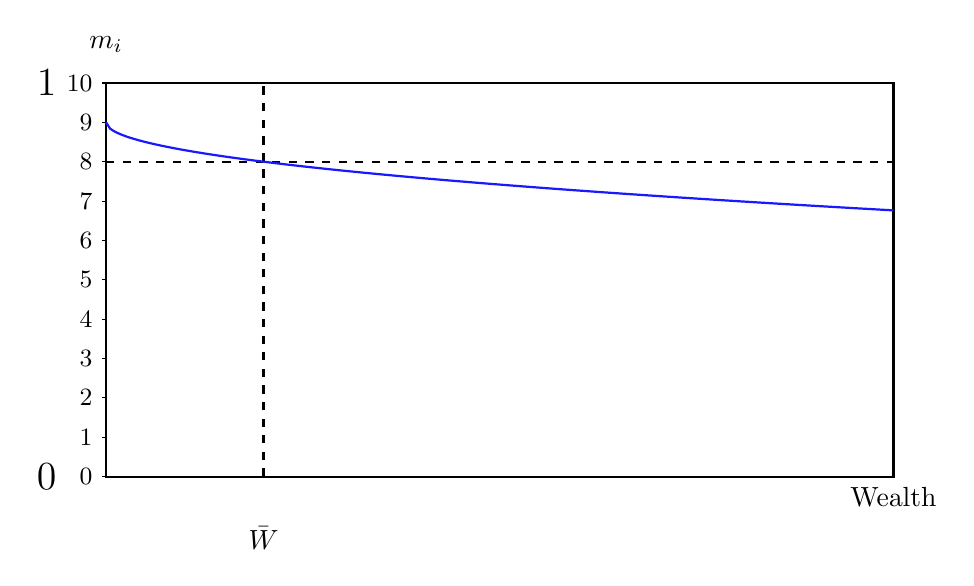
\begin{tikzpicture}[scale=.5]
% \def\bndmax{5}        %https://tex.stackexchange.com/questions/68462/filling-a-complex-region-with-tikz
% \def\bndmin{0.2}
\def\Y{10}  % height of y axis pecent
\def\W{20}  % length  of x axis
\def\Wbar{4}
\def\rbar{8}% this is the prime rate
% Equation   \[ r_i = (A + .5 \frac{\bar{W}}{W_i})\omega\]
% \def\Wmin{.63}  %This sets the lower limit fo the 
\def\Wmin{(\B*\Wbar)/(\Y/\rbar-\A)} %function to keep in in bounds
\tikzset{func/.style={thick,color=blue!90}}	
\draw [thick](\W,\Y)-- (0,\Y)node[left=.5cm]{\Large$1$}node[above=.25cm]{$m_i$} -- (0,0)node[left=.5cm]{\Large$0$}--(\W,0)node[below]{Wealth}--cycle;  	% Axes box
\draw [dashed, thick] (0,\rbar) -- (\W,\rbar);  	% Axes
\draw [thick,dashed] ( \Wbar,0)node[below=.5cm]{$\bar{W}$} -- (\Wbar,\Y);  	% Axes
\foreach \yi in {0,...,\Y} \draw (0,\yi)--(-.1,\yi)node[left]{\small$\yi$};
% \foreach \yi in {0,2,4,6,8,10} \draw (0,\yi)--(-.1,\yi));
% node[left]{\small$\yi$};
% \foreach \yi in {0,2,4,6,8,10}node at (-.1,yi) {{10*yi}} ;
\draw[func,domain=0:\W] plot [samples=200] (\x,(9-\x^.5/2);
\end{tikzpicture}
\end{center}
\caption{Individual borrowing ratio $m_i$ as a function of wealth}
\label{fig-individual-borrowing-rate}
\end{figure}


\subsection{Income-based mortgage maximum}

\begin{align}M^{max\_permitted}_i\ = \frac{\mathrm{ability\_to\_carry\_mortgage}*(\omega+\psi+ r_{prime}* \mathrm{savings})}{r_i}\end{align}\label{eqn-income-based-mortgage}
Where ability to carry a mortgage, is the maximum the bank will let an applicant pay based on their wealth.
 
\subsection{Combined mortgage maximum permitted by the bank for new buyers and second home buyers}

The above  two equations specify two constraints on the mortgage,  combining we get:
\begin{align} 
M_i^{max} &= min \left\{ m_i^{max\_permitted}*P, \ M^{max\_permitted}_i \right\} 
% &= min \left\{ \left(0.9- \left( \frac{W_i}{\bar W}\right)^{0.1}\right)P, \  \frac{0.28*(\omega+\psi)}{r_i} \right\}, 
\label{eqn-max-mortgage-combined}
\end{align}

where small $m_i$ a ratio of income, and capital $M_i$ a maximum dollar value.




\section{Individualized borrowing rates} \label{section-borowing-rate}

The cost of capital differs for rich and poor. We tie the individual cost of capital,  $r_i$ for agent $i$, to The lender's target rate $r^{target}$, and to individual wealth. Figure~\ref{fig-capital-cost} illustrates the cost of the borrowing model we implement, which is  roughly consistent  with the stylized facts about lenders. 
 
\begin{equation}
r_i = r^{target}+ K/(W-W_{min}) -K/(\bar W - W_{min})\label{eqn-interest-wealth-relationship}
\end{equation}
%  \begin{equation}. %.  OLD
% r_i = (A + B \frac{\bar{W}}{W_i})\bar r\label{eqn-interest-wealth-relationship}
% \end{equation}

%  Capital cost equation
 
% \[   r^h=\frac{ \delta(1+\dot p  - (1+r)m) \ + \rho   	-\kappa - t } {1-m}    \]

\begin{figure}[!hb]
\begin{center}

% Large version
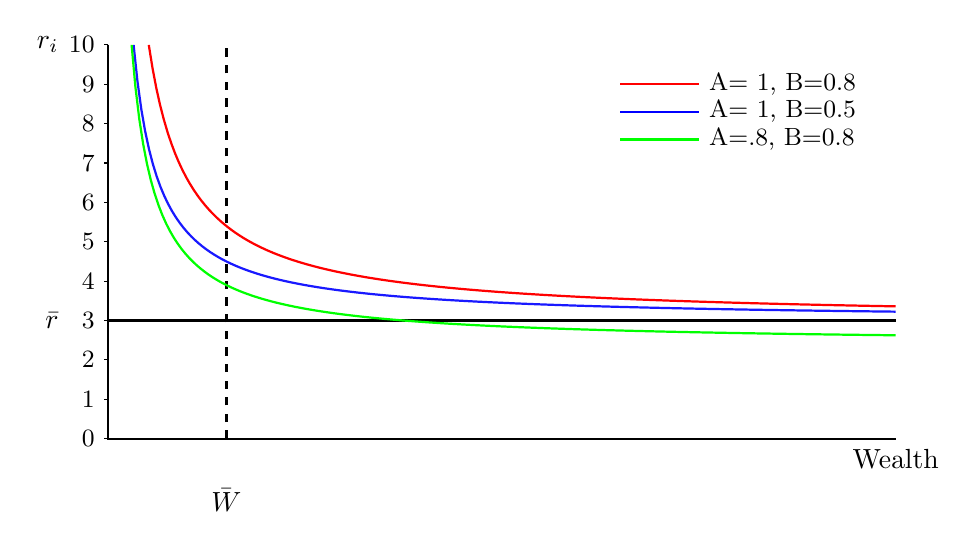
\begin{tikzpicture}[scale=.5]
%\def\bndmax{5}        %https://tex.stackexchange.com/questions/68462/filling-a-complex-region-with-tikz
%\def\bndmin{0.2}
\def \Y {10}  % height of y axis pecent
\def \W {20}  % length  of x axis
\def \Wbar {3} % jmeam wealth
\def \omega {3}
\def \A {1}  %was .5
\def \B {.5}
%Equation   \[ r_i = (A + .5 \frac{\bar{W}}{W_i})\omega\]
\def \Wmin{.63}  %This sets the lower limit fo the 
\def \Wmin{(\B*\Wbar)/(\Y/\omega-\A)} %function to keep in in bounds
	
\tikzset{func/.style={thick,color=blue!90}}	

\draw [thick] (0,\Y)node[left=.5cm]{$r_i$} -- (0,0)--(\W,0)node[below]{Wealth};  	% Axes
\draw [thick] (0,\omega)node[left=.5cm]{$\bar r$} -- (\W,\omega);  	% Axes
\draw [thick,dashed] ( \Wbar,0)node[below=.5cm]{$\bar{W}$} -- (\Wbar,\Y);  	% Axes

\foreach \yi in {0,...,\Y} \draw (0,\yi)--(-.1,\yi)node[left]{\small$\yi$};

\draw[func,domain=\Wmin:\W] plot [samples=200] (\x,{(\A+\B*\Wbar/\x)*\omega});
\def \A {.8}
\draw[func,domain=\Wmin:\W, green] plot [samples=200] (\x,{(\A+\B*\Wbar/\x)*\omega});

\def \A {1}
\def \B {.8}
\draw[func,domain=\Wmin:\W, red] plot [samples=200] (\x,{(\A+\B*\Wbar/\x)*\omega});

\draw [red,  thick](13, 9)--(15,9)node [right, black] {\small A=\ 1,\ B=0.8};
\draw [blue,  thick](13, 8.3)--(15,8.3)node [right, black] {\small A=\ 1,\ B=0.5};
\draw [green, thick](13, 7.6)--(15,7.6)node [right, black] {\small A=.8, B=0.8};
\end{tikzpicture}

% % Small version with equation and parameter values
% \[   r^h=\frac{ \delta(1+\dot p  - (1+r)m) \ + \rho   	-\kappa - t } {1-m}    \]
% \begin{tikzpicture}[scale=.35]
% %\def\bndmax{5}        %https://tex.stackexchange.com/questions/68462/filling-a-complex-region-with-tikz
% %\def\bndmin{0.2}
% \def \Y {10}  % height of y axis percent
% \def \W {18}  % length  of x axis
% \def \Wbar {3} % j mean wealth
% \def \omega {3}
% \def \A {1}  %was .5
% \def \B {.5}
% %Equation   \[ r_i = (A + .5 \frac{\bar{W}}{W_i})\omega\]
% \def \Wmin{.63}  %This sets the lower limit fo the 
% \def \Wmin{(\B*\Wbar)/(\Y/\omega-\A)} %function to keep in in bounds
	
% \tikzset{func/.style={thick,color=blue!90}}	

% \draw [thick] (0,\Y)node[left=.5cm]{$r_i$} -- (0,0)--(\W,0)node[below]{Wealth};  	% Axes
% \draw [thick] (0,\omega)node[left=.5cm]{$\bar r$} -- (\W,\omega);  	% Axes
% \draw [thick,dashed] ( \Wbar,0)node[below=.5cm]{$\bar{W}$} -- (\Wbar,\Y);  	% Axes

% \foreach \yi in {0,...,\Y} \draw (0,\yi)--(-.1,\yi)node[left]{\tiny$\yi$};

% \draw[func,domain=\Wmin:\W] plot [samples=200] (\x,{(\A+\B*\Wbar/\x)*\omega});
% \def \A {.8}
% \draw[func,domain=\Wmin:\W, green] plot [samples=200] (\x,{(\A+\B*\Wbar/\x)*\omega});

% \def \A {1}
% \def \B {.8}
% \draw[func,domain=\Wmin:\W, red] plot [samples=200] (\x,{(\A+\B*\Wbar/\x)*\omega});

% \draw [red,  thick](10, 9)--(12,9)node [right, black] {\tiny A=\ 1,\ B=0.8};
% \draw [blue,  thick](10, 8)--(12,8)node [right, black] {\tiny A=\ 1,\ B=0.5};
% \draw [green, thick](10, 7)--(12,7)node [right, black] {\tiny A=.8, B=0.8};

% \def \W {19}  % length  of x axis
% \node[right] at (\W,9.5){\small$\delta=$discount factor};
% \node[right] at (\W,8.5){\small$\dot p=$appreciation rate};
% \node[right] at (\W,7.5){\small$r=$borrowing rate};
% \node[right] at (\W,6.5){\small$m=$mortgage/price};
% \node[right] at (\W,5.5){\small$\rho=$rental  rate};
% \node[right] at (\W,4.5){\small$\kappa=$op cost rate};
% \node[right] at (\W,3.5){\small$t=$tax rate};
% \node[right] at (\W,2.5){\small$\upsilon=$use value rate};
%  \end{tikzpicture}



% One blue line with x-shift, y-shift
% \begin{figure}
% \begin{tikzpicture}[scale=.5]
% %\def\bndmax{5}        %https://tex.stackexchange.com/questions/68462/filling-a-complex-region-with-tikz
% %\def\bndmin{0.2}
% \def \Y {10}  % height of y axis pecent
% \def \W {20}  % length  of x axis
% \def \Wbar {3} % meam wealth
% \def \rbar {3}% this is the prime rate 

% %\def \Wmin{(\B*\Wbar)/(\Y/\rbar-\A)} %function to keep in in bounds
% \tikzset{func/.style={thick}}	
% 	% Axes
% \draw [thick] (0,\Y)node[left=.5cm]{$r_i$} -- (0,0)--(\W,0)node[below]{Wealth};  
% \foreach \yi in {0,...,\Y} \draw (0,\yi)--(-.1,\yi)node[left]{\small$\yi$};
% \draw [thick] (0,\rbar)node[left=.5cm]{$\bar r$} -- (\W,\rbar);  	% Axes
% \draw [thick,dashed] ( \Wbar,0)node[below=.5cm]{$\bar{W}$} -- (\Wbar,\Y);  	% 

% \def \A {1} %vertical shift aroung \rbar, the prime rate
%  \def \B {1}  % Scales the exponential curveBLUE
%  \def \C {1}  %right shift  
% % \def \Wmin {.4+\B}  %This sets the lower limit fo the 
% \def \Wmin {(\B*\Wbar)/(\Y-\rbar+\A) +\C} %function to keep in in bounds

% \draw[func,domain=\Wmin:\W, color=blue!90] plot [samples=200] (\x,{\rbar-\A+\B*\Wbar/(\x-\C))});
% \node  [align=left, text width =2cm ] at (13, 8.3) {\small y-shift=\A \newline scale=\B \newline x-shift= \C};

%  \end{tikzpicture}
% \caption{Individual borrowing cost as a function of wealth II}
% \label{fig-borrowingrate2}
% \end{figure}

% The rates $\delta,\ \sigma,$ and $r$ depend on the period, $T$. 


% LARGE WITH DIFFERENT PARAMETER VALUES THAN MAOIN FIGURE - MORE SPREAD

% \begin{figure}
% \begin{tikzpicture}[scale=.5]
% %\def\bndmax{5} % https://tex.stackexchange.com/questions/68462/filling-a-complex-region-with-tikz
% %\def\bndmin{0.2}
% \def \Y {10}    % height of y axis as a pecent
% \def \W {20}    % length  of x axis
% \def \Wbar {3}  % mean wealth
% \def \rbar {3}  % the prime rate 

% % Equation   \[ r_i = (A + .5 \frac{\bar{W}}{W_i})\omega\]
% \def \Wmin{.63}  %This sets the lower limit fo the 
% \def \Wmin{(\B*\Wbar)/(\Y/\rbar-\A)} %function to keep in in bounds
% \tikzset{func/.style={thick}}	

% % Axes
% \draw [thick] (0,\Y)node[left=.5cm]{$r_i$} -- (0,0)--(\W,0)node[below]{Wealth};  
% \foreach \yi in {0,...,\Y} \draw (0,\yi)--(-.1,\yi)node[left]{\small$\yi$};
% \draw [thick] (0,\rbar)node[left=.5cm]{$\bar r$} -- (\W,\rbar);  	% Axes
% \draw [thick,dashed] ( \Wbar,0)node[below=.5cm]{$\bar{W}$} -- (\Wbar,\Y);  	% 

% \def \A {1.0}  \def \B {0.5} %BLUE
% \draw[func,domain=\Wmin:\W, color=blue!90] plot [samples=200] (\x,{(\A+\B*\Wbar/\x)*\rbar});
% \draw [ultra thick, color=blue!70 ](13, 8.3)--(15,8.3)node [right, black] {\small A=\A,\ B=\B};

% \def \A {0.5} 
% \def \B {0.5} % GREEN
% \draw[func,domain=\Wmin:\W, color=green] plot [samples=200] (\x,{(\A+\B*\Wbar/\x)*\rbar});
% \draw [thick,  color=green](13, 7.6)--(15,7.6)node [right, black] {\small A=\A, B=\B};

% \def \A {1.0}  \def \B {0.8} % RED
% \draw[func,domain=\Wmin:\W, red] plot [samples=200] (\x,{(\A+\B*\Wbar/\x)*\rbar});
% \draw [thick,  color=red](13, 9)--(15,9)node [right, black] {\small A=\A,\ B=\B};
% % KEY
% \end{tikzpicture}
% \caption{Individual borrowing cost as a function of wealth}
% \label{fig-borrowingrate1}
% \end{figure}
% Figure of cost of borrowing
\caption[Borrowing cost for agents depending on wealth.]{Borrowing cost for agents depending on wealth, with different values for parameters $A$ and $B$ in Equation~\ref{eqn-interest-wealth-relationship}.} %$A=1$  $B=0.5$ (blue);  $A=1$  $B=0.8$ (red), and  $A=.8$  $B=0.8$ (green).}
\label{fig-capital-cost}
\end{center}
\end{figure}

\begin{figure}
\centering

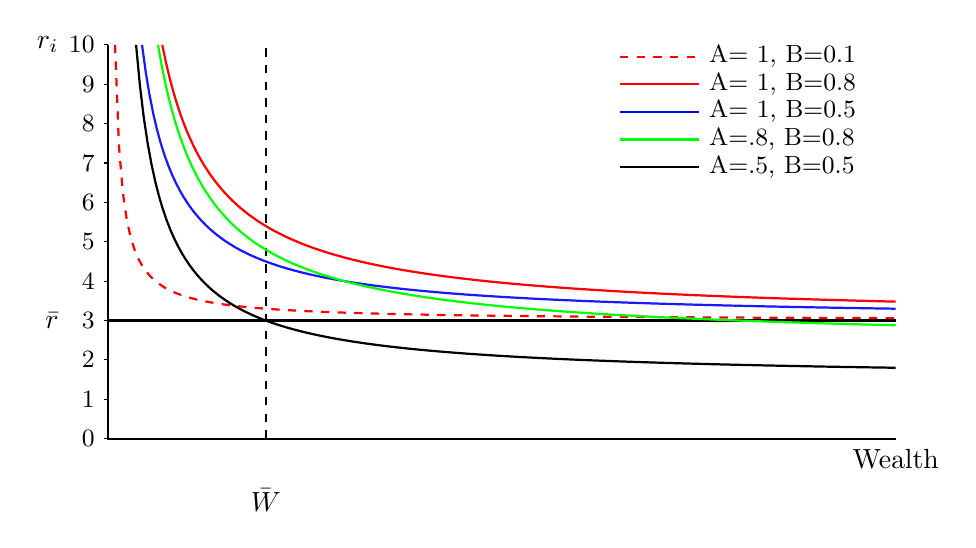
\begin{tikzpicture}[scale=.5]
%\def\bndmax{5}        %https://tex.stackexchange.com/questions/68462/filling-a-complex-region-with-tikz
%\def\bndmin{0.2}
\def \Y {10}  % height of y axis pecent
\def \W {20}  % length  of x axis
\def \Wbar {4} % jmeam wealth
\def \omega {3} % N.B.:  this is r bar

%Equation   \[ r_i = (A + .5 \frac{\bar{W}}{W_i})\omega\]
\def \Wmin{.63}  %This sets the lower limit fo the 
\def \Wmin{(\B*\Wbar)/(\Y/\omega-\A)} %function to keep in in bounds
	
\tikzset{func/.style={thick}}	

\draw [thick] (0,\Y)node[left=.5cm]{$r_i$} -- (0,0)--(\W,0)node[below]{Wealth};  	% Axes
\draw [thick] (0,\omega)node[left=.5cm]{$\bar r$} -- (\W,\omega);  	% Axes
\draw [thick,dashed] ( \Wbar,0)node[below=.5cm]{$\bar{W}$} -- (\Wbar,\Y);  	% Axes

\foreach \yi in {0,...,\Y} \draw (0,\yi)--(-.1,\yi)node[left]{\small$\yi$};

%     ORANGE
% \def \A {1} \def \B {.8}
% \draw[func,domain=\Wmin:\W, orange] plot [samples=200] (\x,{(\A/\x+\B*\X/\Wbar/\x)*\omega});
% \def \A {1} \def \B {.1}
% \draw[func,domain=\Wmin:\W, orange, dashed] plot [samples=200] (\x,{(\A+\B*\X/\Wbar/\x)*\omega});

%     RED
\def \A {1} \def \B {.8}
\draw[func,domain=\Wmin:\W, red] plot [samples=200] (\x,{(\A+\B*\Wbar/\x)*\omega});
\def \A {1} \def \B {.1}
\draw[func,domain=\Wmin:\W, red, dashed] plot [samples=200] (\x,{(\A+\B*\Wbar/\x)*\omega});

%.    BLUE
\def \A {1} \def \B {.5}
\draw[func,domain=\Wmin:\W, blue!90] plot [samples=200] (\x,{(\A+\B*\Wbar/\x)*\omega});
%     GREEN
\def \A {.8} \def \B {.8}
\draw[func,domain=\Wmin:\W, green] plot [samples=200] (\x,{(\A+\B*\Wbar/\x)*\omega});
%.    BLACK
\def \A {.5} \def \B {.5}
\draw[func,domain=\Wmin:\W, black] plot [samples=200] (\x,{(\A+\B*\Wbar/\x)*\omega});


\draw [red,  thick](13, 9)--(15,9)node [right, black] {\small A=\ 1,\ B=0.8};
\draw [red,  thick, dashed](13, 9.7)--(15,9.7)node [right, black] {\small A=\ 1,\ B=0.1};
\draw [blue,  thick](13, 8.3)--(15,8.3)node [right, black] {\small A=\ 1,\ B=0.5};
\draw [green, thick](13, 7.6)--(15,7.6)node [right, black] {\small A=.8, B=0.8};
\draw [black, thick](13, 6.9)--(15,6.9)node [right, black] {\small A=.5, B=0.5};
\end{tikzpicture}


\label{fig-capital-cost}
\caption{Individual borrowing rate $r\_i$ price of capital}
\label{fig:Wealth-based}
\end{figure}

Where  $r^{target}$ is the bank's target rate of return,  $\bar{W}$ is mean wealth and $W_i$ is individual wealth, $W_{min}$ is the level of wealth the bank requires to lend at all, and $K$ is a parameter for the wealth-sensitivity of lending.\footnote{The median after-tax income of Canadian families and unattached individuals was \$66,800 in 2020 according to Statistics Canada.%'s 
%\href{https://www150.statcan.gc.ca/n1/daily-quotidien/220323/dq220323a-eng.htm}{Canadian Income Survey, 2020}.  \href{https://www150.statcan.gc.ca/t1/tbl1/en/tv.action?pid=1110005501}
% Data released in 2020 by Statistics Canada indicates that t
 The top 1\% of reporting Canadians made, on average, around \$512,000 in a single year \cite{WEB_model-stats-can-canadian-incomes}. % \href{https://www150.statcan.gc.ca/n1/daily-quotidien/201222/dq201222b-eng.htm}{Survey of Financial Security, 2019}.
 %A study by Statistics Canada found that t
 The typical Canadian household now has a median net worth of \$329,900, while the average net worth in Canada is \$738,200 \cite{WEB-model-stats-can-median-net-worth}.  %\href{https://www150.statcan.gc.ca/t1/tbl1/en/tv.action?pid=1110005501}{High income tax filers in Canada}
} The denominator in the last two terms is simply wealth above the lender's minimum. The final term ensures that the target rate is charged for borrowers with average wealth.


%The individual cost of capital,  $r_i$ for agent $i$ is tied to a prime rate, $\bar r$ or the bank's target rate, $r^{target}$, and and varies with individual wealth. %Figures~\ref{fig-borrowing-rate1} % and ref{fig-borrowing-rate1} 
%illustratea a  possible  cost-of-borrowing models 

% \begin{align}
%  r_i =  &  \left(A + B \frac{\bar{W}}{W_i}\right) \bar r       \label{eqn-incomeandr1}  \\
%  r_i =  &  \left(\bar r - A + B *\frac{\bar W}{W_i - C}\right) \label{eqn-incomeandr2}  \\
% \end{align}
% Where $\Bar{W}$ is mean wealth and $W_i$ is individual wealth. In Equation~\ref{eqn-incomeandr2},  A determines y-shift, B, the scale, and C the  x-shift for the curve.


